\documentclass{article}
\usepackage{tikz}
\usetikzlibrary{matrix, calc}
\usepackage{enumitem}

\begin{document}

\section*{Demonstration of Excited Plaquettes}

\textbf{Description:} Demonstration of the excited plaquettes. Yellow plaquettes are the excited ones while white plaquettes stay at the ground state of the corresponding plaquette operators. The first figure is a part of a regular surface code case and the state stays at the ground state. When two pairs of defects are created, two pairs of plaquettes, which have the trivalent vertex, will be excited. Moving defects will move the excited plaquettes accordingly with no more excitation created. After fusing the central two defects, the corresponding excitation annihilates, leaving two remaining defects at ends.

\begin{figure}[h]
    \centering
    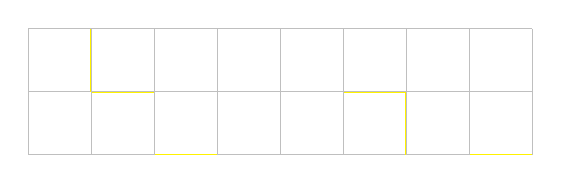
\begin{tikzpicture}[scale=0.8]
        % Draw the grid for the first figure
        \draw[gray!50] (0,0) grid (8,2);

        % Draw the second figure
        \draw[yellow] (1,1) rectangle ++(1,1);
        \draw[yellow] (6,1) rectangle ++(1,1);
        \draw[yellow] (2,0) rectangle ++(1,1);
        \draw[yellow] (7,0) rectangle ++(1,1);

        \foreach \x in {1,...,8} {
            \foreach \y in {1,2} {
                \draw[gray!50] (\x,\y) -- ++(-1,0);
                \draw[gray!50] (\x,\y) -- ++(0,-1);
            }
        }

        % Draw the third figure
        \draw[yellow, dashed] (1,1) -- ++(1,0);
        \draw[yellow, dashed] (1,1) -- ++(0,1);
        \draw[yellow, dashed] (6,1) -- ++(-1,0);
        \draw[yellow, dashed] (6,1) -- ++(0,-1);

        \foreach \x in {1,...,7} {
            \foreach \y in {1,2} {
                \draw[gray!50] (\x,\y) -- ++(1,0);
                \draw[gray!50] (\x,\y) -- ++(0,-1);
            }
        }

        % Draw the fourth figure
        \draw[yellow, thick] (1,1) -- ++(1,0);
        \draw[yellow, thick] (1,1) -- ++(0,1);
        \draw[yellow, thick] (6,1) -- ++(-1,0);
        \draw[yellow, thick] (6,1) -- ++(0,-1);

        \foreach \x in {1,...,7} {
            \foreach \y in {1,2} {
                \draw[gray!50] (\x,\y) -- ++(1,0);
                \draw[gray!50] (\x,\y) -- ++(0,-1);
            }
        }
    \end{tikzpicture}
\end{figure}

\end{document}